\documentclass[12pt,a4paper]{report}
\usepackage[italian]{babel}
\usepackage[utf8]{inputenc}
\usepackage{graphicx}
\usepackage{float}
\usepackage{hyperref}
\usepackage{longtable}
\usepackage{needspace}
\usepackage{amsmath}

\begin{document}

\title{\textbf{ALPHA} 

Acquisizione Locale di Parametri con Hardware Avanzato
}
\author{Alessio Tommasi}
\date{\today}

\maketitle

\tableofcontents

\centering
\chapter{Introduzione}

Il progetto \textit{ALPHA} è stato sviluppato nel corso di IoT del Master in Informatica presso SUPSI. Il focus principale è sull'ESP32 e il protocollo Modbus.

La documentazione ufficiale del progetto disponibile al seguente link: \href{https://progettistudio.supsi.ch/dettaglio.php?p=C10936}{ALPHA}.
\section{Dipendenze}

\paragraph{Driver}
Per gli utenti Windows, è necessario installare \texttt{CP210xDriver}
\paragraph{Compiler}
Per compilare tale progetto e'stato utilizzato Arduino IDE 2.3.3.
disponibile al seguente link: \href{https://www.arduino.cc/en/software}{Arduino IDE}.

\paragraph{Pubblic library}

\subparagraph[short]{AsyncTCP} ulteriori informazioni sono disponibili a questo  \href{https://github.com/dvarrel/AsyncTCP}{link}
\subparagraph[short]{ESPAsyncTCP} ulteriori informazioni sono disponibili a questo  \href{https://github.com/dvarrel/ESPAsyncTCP}{link}
\subparagraph[short]{ESPAsyncWebServer} ulteriori informazioni sono disponibili a questo  \href{https://github.com/dvarrel/ESPAsyncWebSrv}{link}
\subparagraph[short]{UIPEthernet} ulteriori informazioni sono disponibili a questo  \href{https://github.com/UIPEthernet/UIPEthernet}{link}

\paragraph{Modbus} Sono state testate diverse librerie, ma nessuna di esse ha funzionato in modo ottimale.

\section{Configurazione dell'Arduino IDE}

Link repo ufficiale: \href{https://github.com/AlessioTommasi-supsi/iotProject }{iotProject}.

\paragraph{}
Per compilare i file nelle sottocartelle, è necessario aggiungerli come librerie (\texttt{.zip}) all'Arduino IDE. Ho creato una cartella specifica per le librerie dove posizionare o sostituire i file zip. Per una corretta compilazione, importa tutte le cartelle zip presenti in \texttt{/Library}.

\begin{figure}[H]
  \centering
  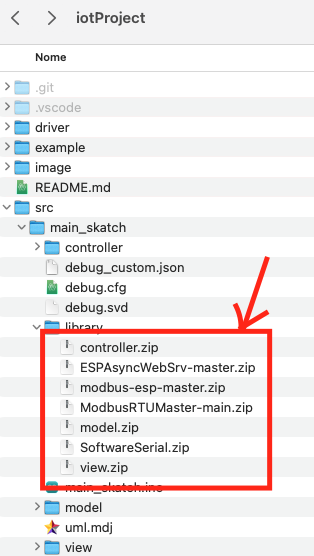
\includegraphics[width=0.3\linewidth]{../image/Library.png}
  \caption{Importazione delle librerie nell'Arduino IDE}
\end{figure}

\paragraph{} Altrimenti clonare la versione Portable del progetto disponibile al seguente link: \href{https://github.com/AlessioTommasi-supsi/iotProject/tree/portable}{iotProject-portable}.


\chapter{Hardware}
\section{Funzionamento}
\subsection{Alimentazione}

E' possibile alimentare la board tramite un alimentatore esterno da 24V DC che fornisca almeno 0.5A.


\begin{figure}[H]
    \centering
    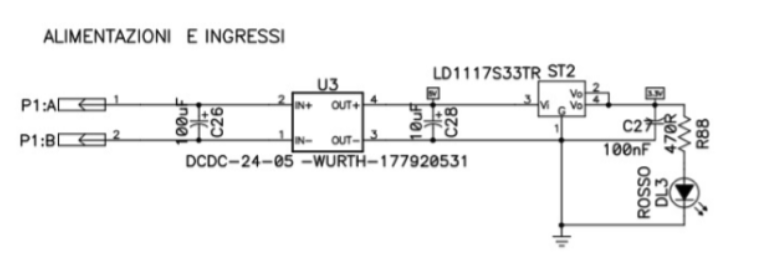
\includegraphics[width=\linewidth]{../image/psu.png}
    \caption{ }
\end{figure}

\paragraph{Descrizione } 
Lo schema in Figura 2.1 
rappresenta il sistema di alimentazione con regolatori di tensione e relativi condensatori di filtraggio. 

I connettori P1:A e P1:B forniscono l'ingresso principale della tensione al circuito.

\paragraph{Conversione DC-DC } 
l primo stadio dell'alimentazione è rappresentato dal modulo DC-DC Wurth 177920531,( \href{https://www.we-online.com/components/products/datasheet/1769205341.pdf}{Data Sheet Here} )
che si occupa della conversione della tensione di ingresso a un livello adeguato per il regolatore successivo. 

La stabilizzazione della tensione è garantita dai condensatori C26 e C28 entrambi da 100 
muF, 
i quali riducono eventuali ripple presenti nella tensione di alimentazione.

\paragraph{Regolazione di tensione}
Dopo la conversione DC-DC, il regolatore lineare 
\href{https://www.mouser.it/datasheet/2/389/ld1117-1849389.pdf}{LD1117S33TR} (U3 sulla board) fornisce una tensione stabile di 3.3V, 
necessaria per l'alimentazione dei componenti successivi. 

Questo regolatore include un condensatore di ingresso C28 di 10uF e 
un condensatore di uscita C27 di 100nF per migliorare la stabilità del segnale.

Un LED rosso (D3) con la resistenza R88 fornisce un'indicazione visiva della corretta alimentazione del sistema.

\paragraph{Regolatore Switching LM7660}
Un ulteriore regolatore di tensione, l'LM7660 (U10), 
viene utilizzato per generare una tensione negativa o fornire una conversione di tensione specifica. 

Questo componente opera con i condensatori C29 e C30 (entrambi da 10uF), i quali servono per stabilizzare la tensione e ridurre le oscillazioni indesiderate.

\paragraph{Uscite}
Le alimentazioni ottenute distribuiti tramite i connettori P20:1, P20:2, P21:1, P21:2, P22:1 e P22:2, 
che permettono l'integrazione del sistema con altri moduli elettronici.

P20:1 e P20:2 forniscono la tensione di alimentazione principale a 5V, mentre P21:1 e P21:2 forniscono la tensione negativa a -5V.

P22:1 e P22:2 forniscono la tensione di alimentazione a 3.3V.

\newpage

\subsection{Ingressi Digitali}

Questo sezione descrive l'implementazione degli ingressi digitali nel circuito, illustrando il principio di funzionamento, la protezione e il filtraggio dei segnali.
\begin{figure}[H]
    \centering
    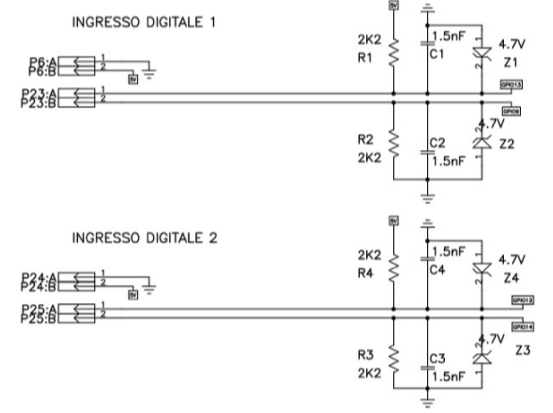
\includegraphics[width=\linewidth]{../image/IngressiDigitali.png}
    \caption{ }
\end{figure}

\paragraph{Descrizione}
Il circuito degli ingressi digitali è progettato per accettare segnali in ingresso e condizionarli adeguatamente prima di inviarli alla logica di elaborazione. 

\textbf{Ogni ingresso è dotato di:}

- \textbf{Resistenze} da 2.2 k$\Omega$
 rispettivamente (R1, R2) per ingresso digitalale 1 e (R3, R4) per ingresso digitale 2: 
il loro scopo è limitare la corrente di ingresso e formare un partitore resistivo.

-\textbf{Condensatori} da 1.5 nF (C1, C2, C3, C4): 
implementati per ridurre il rumore ad alta frequenza e migliorare l'integrità del segnale.

-\textbf{Diodi Zener} da 4.7V (Z1, Z2, Z3, Z4): impiegati per proteggere l'ingresso da sovratensioni accidentali che potrebbero danneggiare i componenti a valle.

\paragraph{Conclusioni}

Grazie all'uso combinato di resistenze, condensatori e diodi di protezione, il circuito è in grado di accettare segnali digitali provenienti da diversi dispositivi, mantenendo una buona immunità al rumore. 

Inoltre, la configurazione utilizzata permette di garantire livelli logici stabili e ben definiti.

Dunque il sistema di ingressi digitali descritto rappresenta una soluzione efficace per la gestione di segnali binari, garantendo protezione, stabilità e robustezza. Questa configurazione assicura un'interfaccia affidabile tra il mondo fisico e il sistema di elaborazione.

\newpage
\subsection{Multiplex}
\paragraph{ }
Il dispositivo di multiplexing riulta essere il \textbf{CD405xB}. \\
sviluppato da Texas Insreumet, link alla documentazione ufficiale: \href{https://www.ti.com/lit/ds/symlink/cd4051b.pdf}{CD405xB}. \\ 

Da cui provengono le seguenti immagini e informazioni:
\begin{figure}[H]
    \centering
    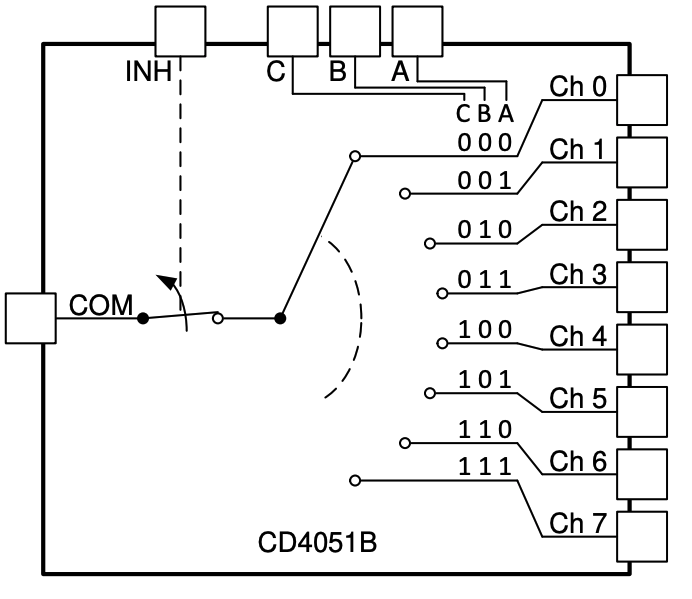
\includegraphics[width=0.5\linewidth]{../image/CD405xB.png}
    \caption{Tabella di verita del CD405xB}
\end{figure}

\subsubsection{Collegamenti Multiplexer}

I pin di ingresso A, B, C del multiplexer \textbf{CD405xB} sono collegati rispettivamente ai pin GPIO 12, 13, 14 dell'ESP32. La selezione dei canali del multiplexer avviene impostando i pin A, B, C come segue:

\begin{table}[H]
    \centering
    \begin{tabular}{|c|c|c|c|}
        \hline
        \textbf{Canale} & \textbf{Pin A} & \textbf{Pin B} & \textbf{Pin C} \\ \hline
        0 & 0 & 0 & 0 \\ \hline
        1 & 1 & 0 & 0 \\ \hline
        2 & 0 & 1 & 0 \\ \hline
        3 & 1 & 1 & 0 \\ \hline
        4 & 0 & 0 & 1 \\ \hline
        5 & 1 & 0 & 1 \\ \hline
        6 & 0 & 1 & 1 \\ \hline
        7 & 1 & 1 & 1 \\ \hline
    \end{tabular}
    \caption{Configurazione dei pin per la selezione dei canali del multiplexer}
\end{table}

i canali del multiplexer possono essere impostati nella apposita pagina web, la documentazione è disponibile piu avanti in questo documento. \\
\hyperref[lbl_webserver]{link alla sezione apposita}

\paragraph{Dettaglio canali multiplexer} 
Di seguito sono riportati come i canali si connettono ai segnali esterni, le operazioni effettuate su tali segnali verranno spiegate piu nel dettaglio nella sezioni successive.

\begin{figure}[H]
    \centering
    \includegraphics[width=\linewidth]{../image/fromMutexToPeripheral.png}
    \caption{Dettaglio canali multiplexer}
\end{figure}

\subsection{ hardware esterno posizionabile sulla board}
\subsubsection{MAX31865}
asd

\begin{figure}[H]
    \centering
    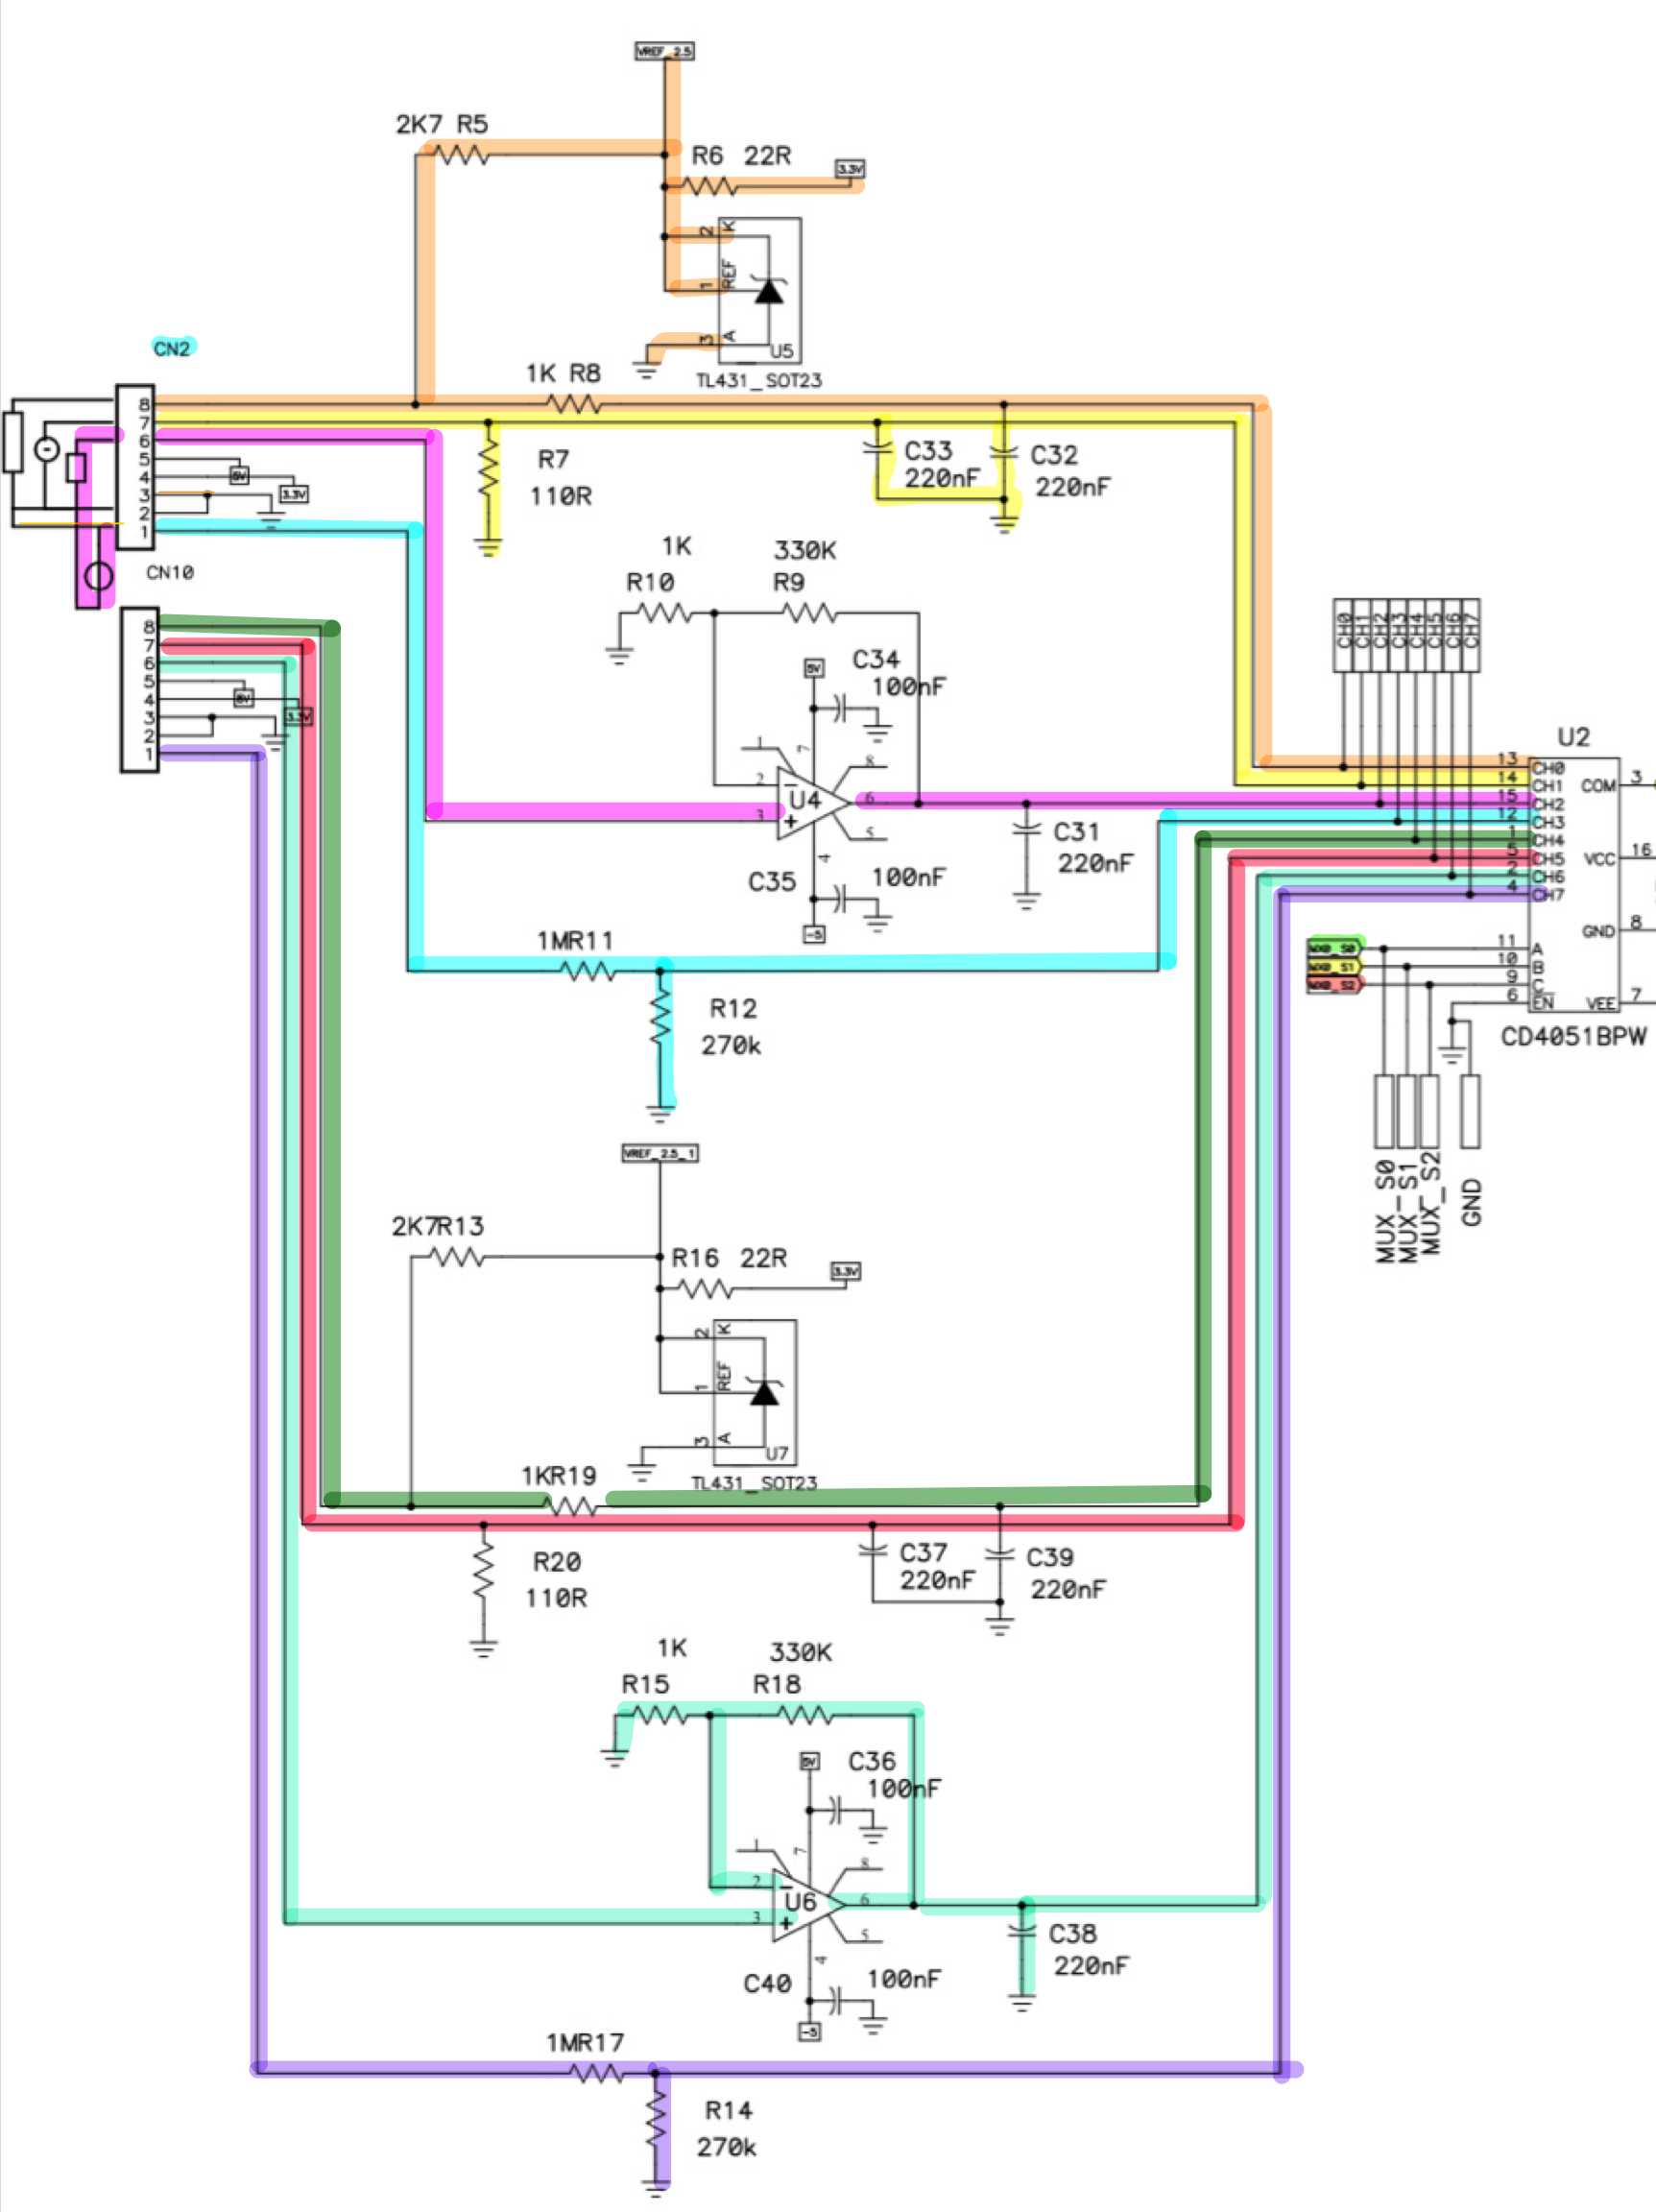
\includegraphics[width=\linewidth]{../image/channelMultiplex.png}
    \caption{Collegamenti dei canali del multiplexer}
\end{figure}

\paragraph{Ch0}
Selezionando Ch0 dall apposita pagina dedicata segue il percorso evidenziato in arancione nella Figura 5.2.
E' collegato a pin 8 della morsettiera CN2.

Il segnale in ingresso proviene da una resistenza esterna collegata al connettore (tra i morsetti 8 e 2 e 1). 

Una corrente di circa 9 µA viene iniettata nel morsetto 8. 

Questa corrente, attraversando la resistenza esterna, genera una caduta di tensione che viene selezionata tramite il canale Ch0 del multiplexer. 

Successivamente, il segnale passa attraverso uno stadio amplificatore per essere portato a un livello adeguato per l'ADC dell'ESP32.

Il componente TL431 funge da riferimento di tensione, ovvero un generatore di tensione costante e calibrata.

\paragraph{Esempio } 
\subparagraph{Dati}

\begin{itemize}
    \item R = 100 $\Omega$ resistenza che vogliamo misurare
    \item I $\approx$ 9 $\mu$A corrente generata internamente sempre in questo range
    \item Vref = 2.5V tensione di riferimento generata dal TL431
\end{itemize}

Si consideri la legge di Ohm:

\[ V = R \cdot I \quad \text{e} \quad R = \frac{V}{I} \]

seguendo KCL (kirchhoff current law) si ottiene che la corrente che passa per la resistenza R8 e pari alla resistenza collegata sul morsetto 8 + la corrente generata dal componente TL431.

dunque la la tensone su ch0 (Vch0 letta da esp a seguito dello stadio di amplificazione) seguendo KVL (kirchhoff voltage law) e' data da: tensione su R8 + tensione su R

svlogendo i calcoli si ottiene che:

\[ R = \frac{Vch0}{Req}  \] 

\paragraph{Ch1}
percorso evidenziato in giallo nella Figura 5.2.

Possibili funzioni del segnale sul segnale in ingreso al pin 7 della morsettiera CN2.

- \textbf{Filtro Passa Basso}
Se il segnale applicato su R7 è una tensione alternata (AC), il circuito potrebbe attenuare le alte frequenze, lasciando passare solo le frequenze più basse

- \textbf{Stabilizzazione del segnale}

\paragraph{Ch2}
percorso evidenziato in viola nella Figura 5.2.

Leggeremo il segnale in ingresso al pin 6 della morsettiera CN2.

Il segnale verra amplificato dall operazionale U4 che e collegato come amplificatore non invertente (maggiori info al link \href{https://elettronicasemplice.weebly.com/amplificatore-operazionale-non-invertente.html}{LM358}).

Il guadagno di U4 e' dato dalla formula $G = 1 + \frac{R9}{R10}= 1+330 = 331 $.

inoltre tali alimentatore e alimentato tra 0 e +5v quindi clampera il segnale in ingresso tra 0 e +5v.
Il condensatore C31 si occupa di stabilizzare il segnale in uscita.

\paragraph{Ch3}
percorso evidenziato in azzurro nella Figura 5.2.

Leggeremo il segnale in ingresso al pin 1 della morsettiera CN2.

tra il segnale sul pin 1 ed ESP e'presente un partitore di tensione composto da R11 = 1M e R12 = 270K dunque $Vesp = Vpin1 * \frac{R12}{R11+R12} = Vpin1 * \frac{270}{1270} = Vpin1 * 0.2126$.

//correzione:
Si necessita di montare una resistenza tra il pin 8 e il pin 1 della morsettiera CN2.
Vine generata una corrente pari a 9 $\mu$A che passa attraverso la resistenza esterna paria 100 $\Omega$
tale segnale finisce dunque su ch3 dopo essere passato attraverso ad un partitore di tensione.

\paragraph{Esempio}
\subparagraph{Dati}
\begin{itemize}
    \item R = 100 $\Omega$ resistenza collegata al pin 1,8
    \item I $\approx$ 925 $\mu$A 
\end{itemize}

Vr = I * R = 925 $\mu$A * 100 $\Omega$ = 92,5 mV

Successivamente e' presente un partitore resistivo per abbassare la tensione a valori accettabili per l'ESP32 (max 3V).
in particolare: 

\[ Vch3 = Vr12 = Vin * \frac{R12}{R11+R12} = 92,5 [mV] * \frac{1M}{270k} = 19,425 [mV] \]

Dunque fattore di divisio ne del partitore e' 
\[Vch3/Vin = 19,425/92,5 = 0,21 \]

A valle del partitore il componente TL082 si occupa dello stadio di amplificazione.
Questo stadio consente anche una traslazione del segnale nel caso in cui la tensione in ingresso sia negativa offettuando opportuni shift di tensione.

Tale shift viene sempre effettuato in modo di portare il segnale a circa la meta della dinamica dell esp ovvero 1.25V.

\paragraph{Recap sull elaborazione del segnale}
\begin{itemize}
    \item generazione corrente  I $\approx$ 925 $\mu$A che passa attraverso la resistenza esterna
    \item tensione generata Vr = R *I viene ridimensionata da partitore con fattore pari a 0.21
    \item shift dell segnale a 1.25V
\end{itemize}

Questo concetto verra applicato per utilizzare termoresistori (Pt100, Pt1000, Pt500, Ni500) e termocoppie che verranno attaccate e il valore di tensione misurato sara corrispondente a un certo valore di resistenza.

Le sonde di temperatura di questa famiglia però non sono lineari quindi andrà implementata una opportuna tabella di linearizzazione


\paragraph{Utilizzo ch3 per segnali in tensione continua}
l’ingresso per tali segnali è dal pin 1 (positivo) e 2 (negativo ) della morsettiera CN2.

\subparagraph{Esempio}

\[  
    Vin = 10V   
       => 10V * 0.21 = 2.1V
       => 2.1V + 1.25V = 3.35V
\]

Contrariamente al caso precedente, non e' necessario effettuare linearizzazione con tabella poiche il segnale e gia lineare.
Dovro dare dunque un opzione lato SW per selezionare il tipo di segnale in ingresso su CH3. 

Ovvero su ch3 leggero 1.25 quando saranno applicati 0V nella morsettiera CN2 e 3.3V quando ci sono 10V 

\paragraph{Utilizzo ch3 per segnale di corrente}
il generatore di corrente dovra essere inserito tra il pin 7(positivo) e 2(negativo) della morsettiera CN2.

\subparagraph{Esempio}

Consideriamo un generatore di corrente in ingresso di 20mA.

La corrente cadrà sulla resistenza R7 generando una tensione che verrà poi shiftata di 1.25V

0.02mA *110Ohm = 2.2V + 1.25 = 3.45V 

Dunque su ch3 leggero 3.45V quando ci sono 20mA in ingresso.

Ultimo caso è quello delle sonde termocoppie. In questo caso la sonda è inserita tra pin 6 e pin 2

Il multiplexer sarà in posizione ch2

Queste sonde forniscono in uscita al variare della temperatura una tensione di pochi millivolt per questo il segnale deve essere amplificato tramite op177 che è un operazionale a basso offset (ovvero non introduce rumore sul segnale misurato).

Il gain dell’operazionale con queste resistenze è pari a 101 quindi il segnali in ingresso verrà amplificato per 101 volte e shiftato sempre di 1.25V

\paragraph{Ch4}
Connessione equivalente a CH0 

\paragraph{Ch5}
Connessione equivalente a CH1

\paragraph{Ch6}
Connessione equivalente a CH3

Tutte le connessioni equivalenti hanno un circuito hw separato per garantire la massima indipendenza tra i canali.
\section{ Hardware esterno }

\subsection{Winzet W5500 Ethernet module}
tale dispositivo e opzionale e deve essere collocato sulla board in alternativa alla scheda SD.

\begin{figure}[H]
    \centering
    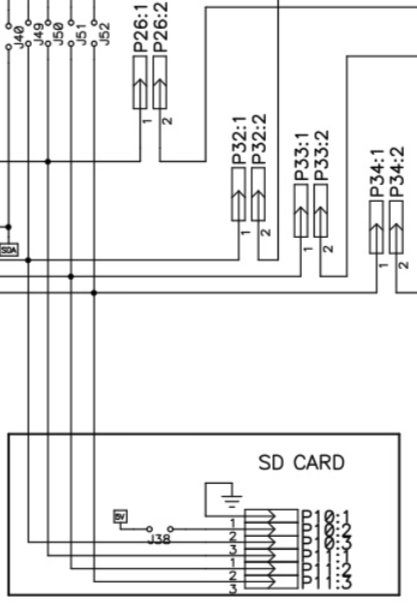
\includegraphics[width=0.7\linewidth]{../image/SD_and_W5500.png}
    \caption{Winzet W5500 Ethernet module}
\end{figure}

per il corretto funzionamento si devono collocare manualmente sullla board seguenti jumper: J49, J50, J51, J52 e J38 visibili in figuras 2.5.

\Needspace{5\baselineskip}

Per una documentazione dettagliata sulla ricerca di tale modulo e sul codice e librerie utilizzate da esso consultare il seguente 

link: \href{https://github.com/AlessioTommasi-supsi/iotProject/blob/main/docs/ResearchEthModule/W5500Example/README.md}{W5500}.

Si e optato per l'utilizzo di un modulo Ethernet W5500 per la comunicazione tramite Modbus TCP/IP.

- documentazione dettagliata modbus tcp/ip \href{https://www.modbus.org/docs/Modbus_Messaging_Implementation_Guide_V1_0b.pdf}{Modbus TCP/IP}

\subsubsection{funzionamento modbus TCP/IP }
Modbus TCP è stato sviluppato per sfruttare le infrastrutture di rete LAN esistenti, permettendo la comunicazione attraverso reti Ethernet. Attualmente viene utilizzato per qualsiasi connessione tra dispositivi connessi a internet.

Questo protocollo incapsula i messaggi Modbus RTU in pacchetti TCP, il che facilita la loro trasmissione su reti Ethernet standard. Uno dei principali vantaggi del Modbus TCP è la sua capacità di connettere un numero illimitato di dispositivi, grazie all’uso di indirizzi IP invece delle limitazioni di indirizzamento dei protocolli seriali.

In questo contesto, Modbus TCP ridefinisce la relazione master-slave in termini di client-server, permettendo una comunicazione più flessibile e scalabile. I dispositivi possono agire come client o server, facilitando l’integrazione di più sistemi e migliorando l’efficienza delle comunicazioni nelle reti industriali.

link bibiografia \href{https://v2charge.com/it/che-cose-modbus-rtu-tpc/}{Modbus TCP/IP}

\subsubsection{Vantaggi W5500}
\begin{itemize}
    \item \textbf{Alta velocità e prestazioni}: Supporta fino a 80 Mbps grazie al buffer hardware dedicato.
    \item \textbf{Stack TCP/IP hardware integrato}: Libera risorse sul microcontrollore ESP32.
    \item \textbf{Consumo energetico ridotto}: Più efficiente rispetto all’ENC28J60, ideale per applicazioni a basso consumo.
    \item \textbf{Compatibilità ampia}: Supportato dalla libreria Ethernet ufficiale di Arduino.
\end{itemize}

Per visualizzare una ricerca piu dettagliata sul confronto di tale modulo con altri moduli presenti sul mercato consultare il seguente link: \href{https://github.com/AlessioTommasi-supsi/iotProject/tree/main/docs/ResearchEthModule}{ResearchEthModule}.

\subsection{MAX485 Modbus RTU} 

Tale moduli sono utilizzati per la comunicazione seriale tra ESP32 e altri dispositivi che supportano il protocollo Modbus RTU.

il dispositivo deve essere alimentato con 5V e collegato ai pin RX e TX dell'ESP32.
per far si che la comunicazione funzioni correttamente collegare cavo trasporto dati dell usb e collegare al dispositivo Master o slave.


\begin{figure}[H]
    \centering
    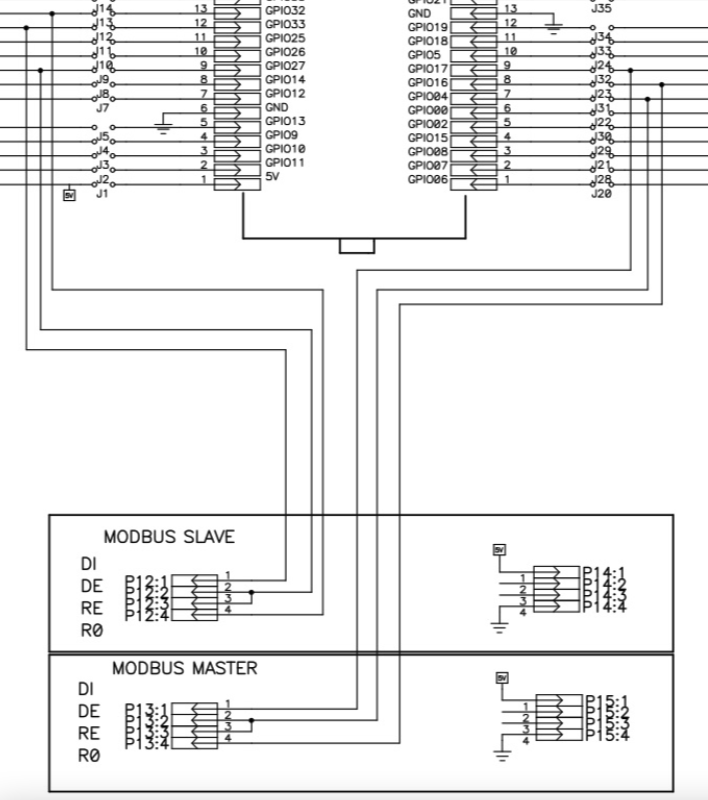
\includegraphics[width=0.9\linewidth]{../image/ModbusWiring.png}
    \caption{MAX485 Modbus RTU}
\end{figure}

\subsubsection{Descrizione Protocollo Modbus RTU}
Modbus RTU è basato su una comunicazione seriale asincrona, che consente la trasmissione di dati su cavi.

Per una corretta comunicazione il dispositivo MAX485 SLAVE deve essere collegato su P12 mentre il dispositivo MASTER su P13.

i collegamenti ai pin dell esp sono rappresentati in figura 2.6.

\begin{itemize}
    \item \textbf{Caratteristiche}
    \begin{itemize}
        \item Formato di messaggio compatto: I messaggi sono compatti, il che consente una trasmissione più rapida ed efficiente.
        \item Modalità binaria: I dati vengono trasmessi in un formato binario, il che significa che si usano bit (0 e 1).
    \end{itemize}
    \item \textbf{Vantaggi del Modbus RTU}
    \begin{itemize}
        \item Ideale per distanze brevi e medie.
        \item Semplice ed economico per installazioni piccole o medie.
    \end{itemize}
    \item \textbf{Limitazioni del Modbus RTU}
    \begin{itemize}
        \item Limitazioni di distanza e velocità.
        \item Numero limitato di dispositivi che possono essere collegati sulla stessa linea di comunicazione, ovvero 32 dispositivi.
    \end{itemize}
\end{itemize}

\newpage

\subsection{ADS1115 ADC}
Il modulo ADS1115 è un convertitore analogico-digitale (ADC) a 16 bit con quattro canali di ingresso.

\begin{figure}[H]
    \centering
    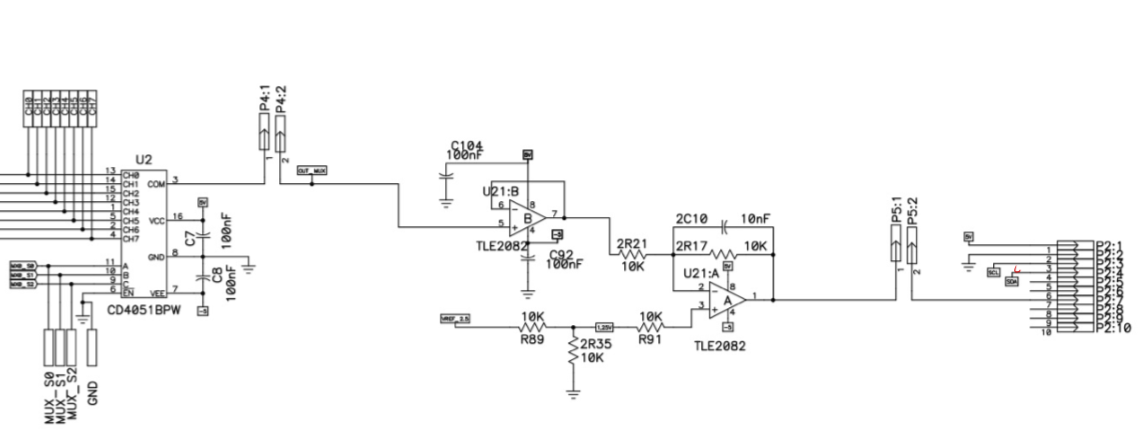
\includegraphics[width=\linewidth]{../image/ADC.png}
    \caption{ADS1115 ADC}
\end{figure}

Il dispositivo utilizza un multiplexer descritto nella sezione  2.1.3  per selezionare uno dei canali di ingresso, amplifica il segnale tramite il PGA e poi lo converte in un valore digitale. 

Il risultato della conversione viene inviato al microcontrollore tramite l'interfaccia I2C.

il datasheet dettagliato di tale dispositivo e' disponibile al seguente link: \href{https://www.ti.com/lit/ds/symlink/ads1115.pdf}{ADS1115}.

\textbf{Pin per tresferimento dati}:

Il collegamento SCL dell ADS una volta collegato il jumper J39 si collega a PIN39 ovvero GPIO 22 

Il collegamento SDA dell ADS una volta collegati il jumper J40 si collega al pin GPIO 21

\newpage
\subsection{ESP32 38 Pin}
\subsubsection{Descrizione}
L'ESP32 è un potente microcontrollore prodotto da Espressif Systems che integra funzionalità Wi-Fi e Bluetooth, rendendolo ideale per applicazioni IoT (Internet of Things), automazione domestica, sistemi indossabili, monitoraggio remoto e molti altri progetti. 

La versione a 38 pin offre una vasta gamma di GPIO (General Purpose Input/Output) utilizzabili per diversi scopi.

\textbf{Caratteristiche principali}:
\begin{itemize}
    \item \textbf{Dual-core Tensilica LX6}: Processore dual-core con velocità di clock fino a 240 MHz.
    \item \textbf{Wi-Fi e Bluetooth}: Supporto per Wi-Fi 802.11b/g/n e Bluetooth v4.2 BR/EDR e BLE (Bluetooth Low Energy).
    \item \textbf{Interfacce Multiple}: Include SPI, I2C, I2S, UART, ADC, DAC, PWM, e touch sensor.
    \item \textbf{Basso Consumo Energetico}: Modalità di basso consumo per applicazioni a batteria.
    \item \textbf{Memoria Integrata}: SRAM da 520 KB e supporto per memoria esterna.
\end{itemize}

Link alla documentazione ufficiale: \href{https://www.espressif.com/sites/default/files/documentation/esp32-wroom-32_datasheet_en.pdf}{ESP32}.

\begin{figure}[H]
    \centering
    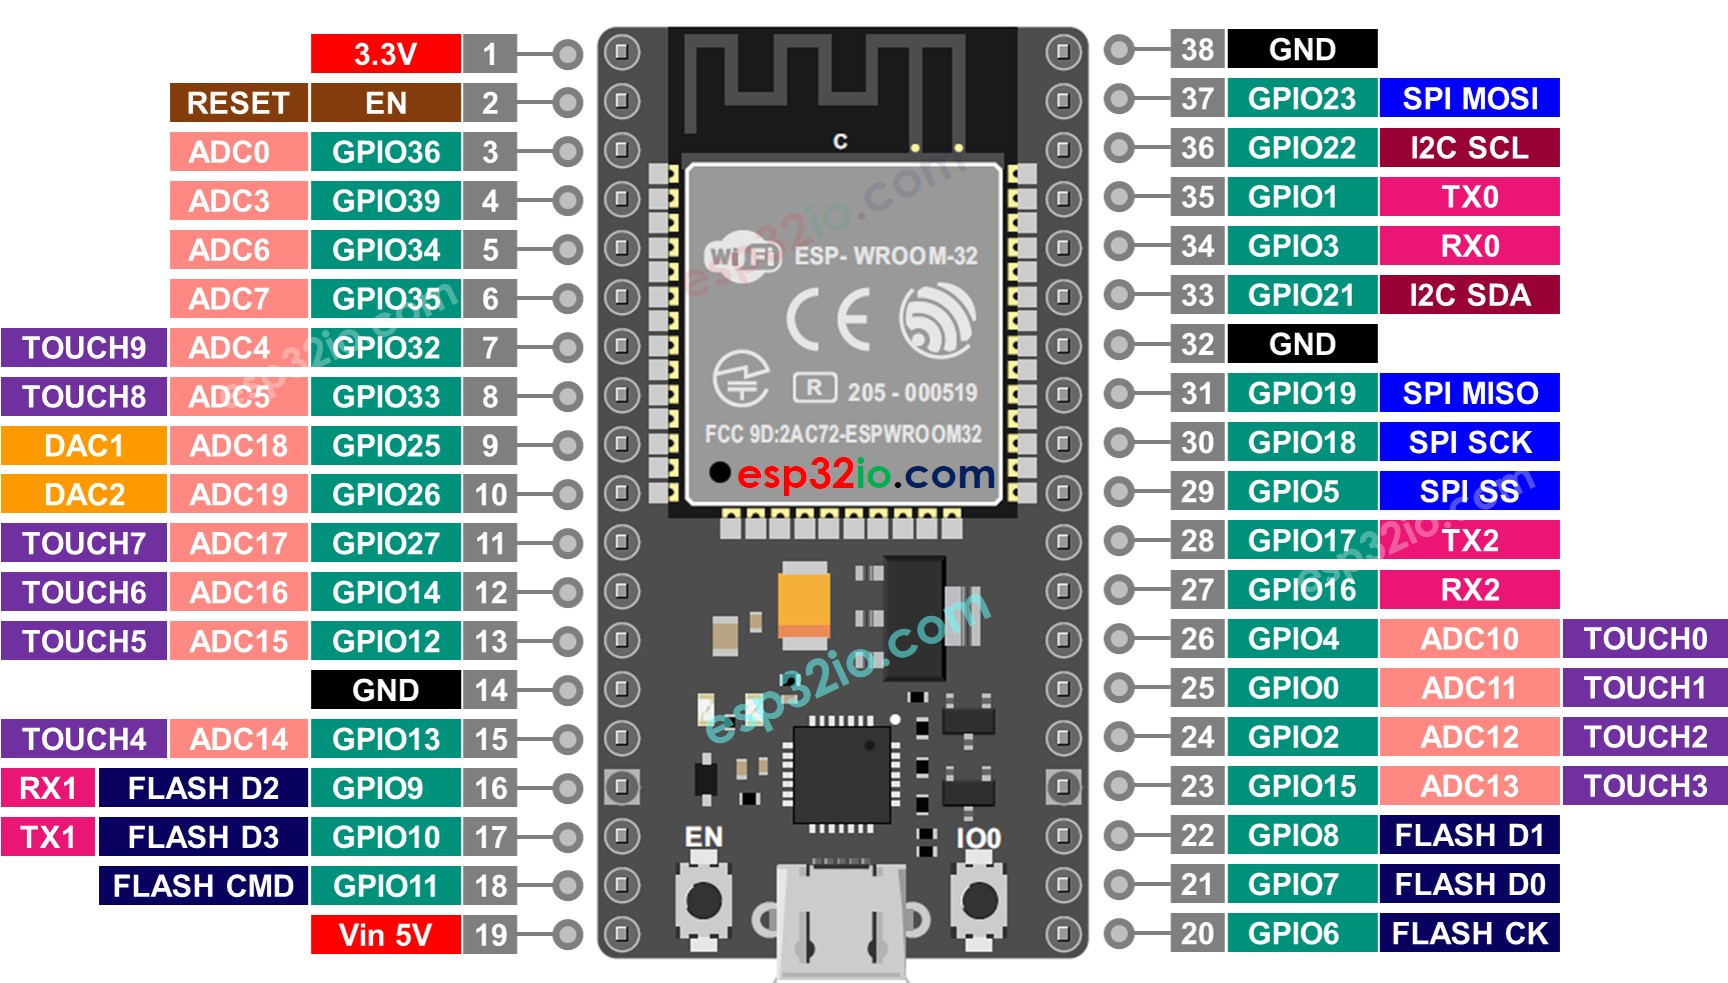
\includegraphics[width=\linewidth]{../image/ESP-38Pin-pinout.jpg}
    \caption{Pinout dell'ESP32-DOIT-DEV-KIT v1}
\end{figure}


\begin{figure}[H]
    \centering
    \includegraphics[width=\linewidth]{../image/collegamenti_daESP.png}
    \caption{collegamenti all'ESP32-DOIT-DEV-KIT v1}
\end{figure}

\begin{table}[H]
    \centering
    \caption{Pinout dell'ESP32 (Versione a 38 pin)}
    \label{tab:esp32_pinout}
    \begin{tabular}{|c|c|c|p{8cm}|}
        \hline
        \textbf{GPIO} & \textbf{Input} & \textbf{Output} & \textbf{Notes} \\ \hline
        0 & pulled up & OK & outputs PWM signal at boot, must be LOW to enter flashing mode \\ \hline
        1 & TX pin & OK & debug output at boot \\ \hline
        2 & OK & OK & connected to on-board LED, must be left floating or LOW to enter flashing mode \\ \hline
        3 & OK & RX pin & HIGH at boot \\ \hline
        4 & OK & OK & \\ \hline
        5 & OK & OK & outputs PWM signal at boot, strapping pin \\ \hline
        6 & x & x & connected to the integrated SPI flash \\ \hline
        7 & x & x & connected to the integrated SPI flash \\ \hline
        8 & x & x & connected to the integrated SPI flash \\ \hline
        9 & x & x & connected to the integrated SPI flash \\ \hline
        10 & x & x & connected to the integrated SPI flash \\ \hline
        11 & x & x & connected to the integrated SPI flash \\ \hline
        12 & OK & OK & boot fails if pulled high, strapping pin \\ \hline
        13 & OK & OK & \\ \hline
        14 & OK & OK & outputs PWM signal at boot \\ \hline
        15 & OK & OK & outputs PWM signal at boot, strapping pin \\ \hline
        16 & OK & OK & \\ \hline
        17 & OK & OK & \\ \hline
        18 & OK & OK & \\ \hline
        19 & OK & OK & \\ \hline
        21 & OK & OK & \\ \hline
        22 & OK & OK & \\ \hline
        23 & OK & OK & \\ \hline
        25 & OK & OK & \\ \hline
        26 & OK & OK & \\ \hline
        27 & OK & OK & \\ \hline
        32 & OK & OK & \\ \hline
        33 & OK & OK & \\ \hline
        34 & OK &  & input only \\ \hline
        35 & OK &  & input only \\ \hline
        36 & OK &  & input only \\ \hline
        39 & OK &  & input only \\ \hline
    \end{tabular}
\end{table}
    
    

\chapter{Software}
\section{Diagramma UML}
\begin{figure}[H]
    \centering
    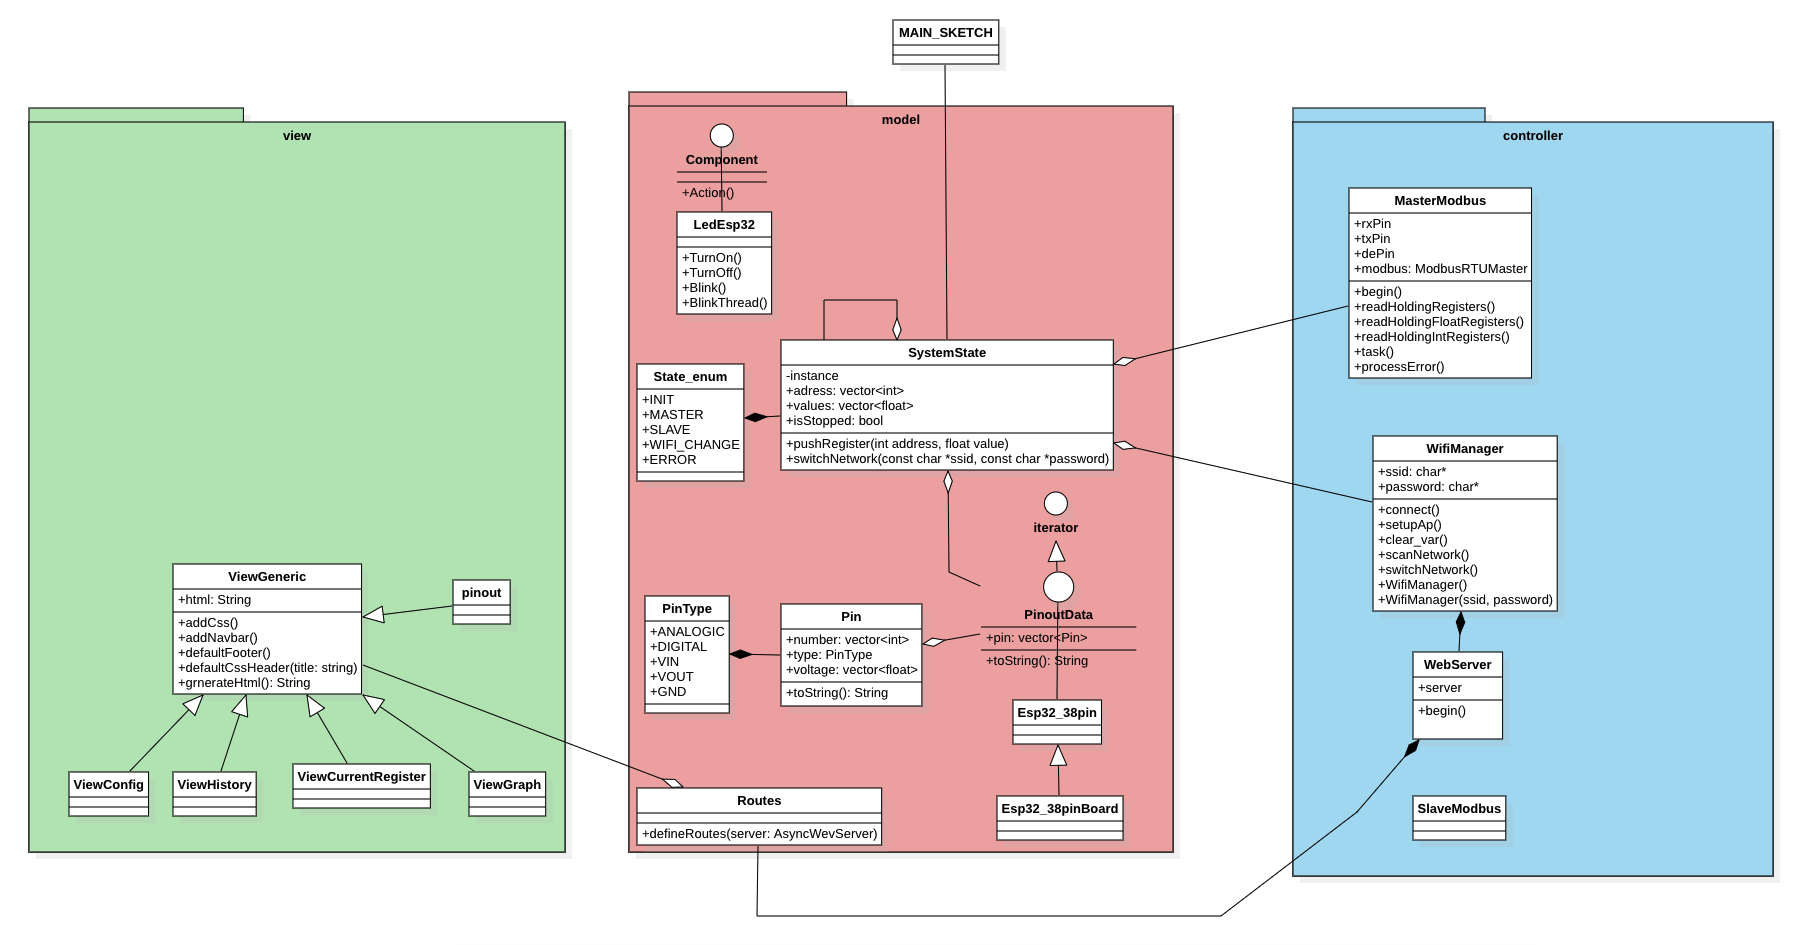
\includegraphics[width=\linewidth]{../image/uml.png}
    \caption{Diagramma UML del sistema}
\end{figure}
\subsection{Pattern}
\subsubsection{Model-View-Controller (MVC)}
\paragraph{Model} Contiene la struttura dei dati e le funzioni per accedere e modificarli. 
Le classi coinvolte sono \texttt{SystemState}, \texttt{Pin}, \texttt{PinoutData}, \texttt{Routes}.
\paragraph{View} Si occupa di visualizzare i dati e di interagire con l'utente.

principalmente sono classi che si occupano della generazione dei componenti delle pagine web visualizzate dall utente.

\paragraph{Controller} Gestisce le richieste dell'utente e aggiorna il modello di conseguenza.

\subsubsection{Singleton}
utilizzato per garantire unicita e atomicita dei dati \texttt{SystemState} e'la classe che implementa tale pattern.
Sara particolarmente utile in futuro per l'implementazione di un sistema di datalogging e persistenza dei dati su scheda SD.

Dallo sketch principale e inoltre possibile definirsi una Board custom estendendo la classe pinout e un wifi di default sulla quale connettersi senza dover passare ogni volta dall AP dell esp per garantirne una migliore usabilita.


\section{Performace}

Il programma caricato ottiene i seguenti risultati dal compilatore integrato ad Arduino IDE:
\begin{verbatim}
    Sketch uses 1291045 bytes (98%) of program storage space.
     Maximum is 1310720 bytes.
    Global variables use 50448 bytes (15%) of dynamic memory, 
    leaving 277232 bytes for local variables. 
    Maximum is 327680 bytes.
\end{verbatim}

\paragraph{Considerazioni: }

Analizzanto tale outputse ne deduce che il programma utilizza il 98\%
dello spazio di memorizzazione disponibile. 

Questo elevato utilizzo della memoria flash implica un margine limitato per l'aggiunta di nuove funzionalità o librerie.

l'utilizzo delle variabili globali è pari al 15\% della memoria disponibile, lasciando un ampio margine per le variabili locali e altre strutture di dati dinamici.

Questa situazione è favorevole, in quanto garantisce la flessibilità necessaria per gestire strutture dati complesse e consentire allocazioni dinamiche.

 

Dunque , per garantire la stabilità e l'espandibilità del progetto, potrebbe essere utile considerare l'acquisto di una versione dell'ESP32 con una maggiore capacità di memoria flash disponibile in commercio. 

Oppure in alternativa, si puo optare per la modifica  lo schema di partizionamento dell'ESP32 per allocare più memoria al codice del programma, riducendo lo spazio destinato alla memoria Dinamica. 

Questa personalizzazione permette di adattare la memoria disponibile alle specifiche esigenze del progetto senza introdurre costi aggiuntivi.


\paragraph{Monitor}
Per un controllo più granulare delle metriche come stack e heap del dispositivo, è stata creata una pagina dedicata che permette il monitoraggio in tempo reale senza impattare sulle prestazioni.

\section{WebServer}
È stato sviluppato un framework estendendo la libreria \href{URL}{AsynkWebsrwerver} per la gestione delle pagine web e delle richieste HTTP.
 tale framework consente di aggiungere dinamicamente componenti HTML alle pagine in base alle richieste del client. 
 
 Questo approccio garantisce una struttura uniforme e un tema coerente che si adatta a tutti i dispositivi.

Il framework è progettato per essere estensibile e modulare. Per aggiungere una nuova pagina, è sufficiente estendere la classe \texttt{ViewGeneric} e aggiungere i componenti desiderati. I nuovi componenti erediteranno automaticamente il tema dell'applicativo, assicurando un aspetto e una sensazione coerenti in tutto il sistema.

\newpage

\subsection{Componenti HTML Dinamici}
Il framework consente di definire componenti HTML come stringhe e di aggiungerli dinamicamente alle pagine web. Questo approccio permette di creare interfacce utente flessibili e reattive.

\subsubsection{Esempio di Aggiunta di una Pagina}
Per aggiungere una nuova pagina al WebServer, è necessario seguire questi passaggi:
\begin{enumerate}
    \item Estendere la classe \texttt{ViewGeneric}.
    \item Definire i componenti HTML desiderati come stringhe.
    \item Aggiungere i componenti alla pagina utilizzando i metodi forniti dal framework.
\end{enumerate}


\begin{verbatim}
    class ViewConfig : public ViewGeneric
    {
    public:
        static String generateHTML(std::vector<std::string> ssidList);
        static String generateHTML();
    
        static String generateComponents(std::vector<std::string> &networks); //Componente che vogliamo aggiungere alla pagina
    };
\end{verbatim}


\begin{verbatim}
    #include "viewConfig.h"

    String viewConfig::html = "";
    
    String viewConfig::generateListComponents( std::vector<std::string> &networks)
    {
        /*Example of a component*/
        String html = "<div class='form-container'>";
        html += "<form action='/switch_wifi' method='get'>";
        html += "<label for='network'>Select Network:</label>";
        html += "<select id='ssid' name='ssid' required>";
    
        for (const std::string &network : networks)
        {
            html += "<option value='" + String(network.c_str()) + "'>" + String(network.c_str()) + "</option>";
        }
    
        html += "</select>";
        html += "<label for='password'>Password:</label>";
        html += "<input type='password' id='password' name='password' required>";
        html += "<button type='submit'>Connect</button>";
        html += "</form>";
        html += "</div>";
    
        return html;
    }
    
    String viewConfig::generateHTML(std::vector<std::string> ssidList)
    {
        String html = viewGeneric::defaultCssHeader("Config Page");
    
        html += viewConfig::generateListComponents(ssidList);

        html += viewComponent2::generate();

        ...
        html += viewComponentN::generate();
    
        html += viewGeneric::defaultFooter();
    
        return html;
    }
    

\end{verbatim}


\paragraph{Routes }
Una volta definito il componente, è necessario aggiungerlo alle route desiderate per poterlo visualizzare.

Questo può essere fatto in due modi:
1. Estendendo il file `Routes.h` e aggiungendo la nuova route.
2. Aggiungendo la route direttamente nel file `Routes.cpp` come segue:

\begin{verbatim}
    void Routes::addRoutes()
    {
        
        server.on("/new_component_routes", HTTP_GET, [](AsyncWebServerRequest *request) {
            String htmlContent = viewConfig::generateHTML(SystemState::getInstance()->wifiManager->scanNetworks());
            const char *htmlContentPtr = htmlContent.c_str();
            request->send(200, "text/html", htmlContentPtr);
        });
    
        ...
    }
\end{verbatim}

\subsection{Vantaggi del Framework}
\begin{itemize}
    \item \textbf{Uniformità}: Garantisce un aspetto e una sensazione coerenti in tutto il sistema.
    \item \textbf{Modularità}: Facilita l'aggiunta di nuove pagine e componenti senza modificare il codice esistente.
\end{itemize}

\subsection{Conclusioni}
Il framework per il WebServer rappresenta una soluzione robusta e flessibile per la gestione delle interfacce web. La sua architettura modulare e la capacità di aggiungere dinamicamente componenti HTML rendono il sistema facile da mantenere e espandere, garantendo al contempo un'esperienza utente coerente e reattiva.

\section{Modbus}
Questa funzionalita non riulta attualmente perfettamente funzionante quindi sara rivista nelle attivita future.
Sono stati fatti diversitentatitivi ognuno di essi e consultabile al seguente link: \href{../src/SLAVE_EXAMPLE/}{Modbus}.


\section{Sfide}
Una delle attività più complesse è stata la gestione dell'accesso concorrente alle variabili da parte delle richieste HTTP asincrone.

È stato necessario implementare una logica che garantisse un accesso atomico alle variabili e una sincronizzazione in tempo reale di tali variabili su più dispositivi.



\chapter{Attività}

\begin{longtable}{|p{0.35\textwidth}|p{0.65\textwidth}|}
\hline
\textbf{Attività} & \textbf{Descrizione} \\ \hline
\endfirsthead
\hline
\textbf{Attività} & \textbf{Descrizione} \\ \hline
\endhead
\hline
\endfoot
\textbf{Configurazione sensori di temperatura} & Configurare e integrare sensori di temperatura \textbf{PT100}, \textbf{PT1000} e \textbf{termocoppie} utilizzando moduli come \textbf{MAX31865} e \textbf{MAX31855}.

 implementazione una opportuna tabella di linearizzazione per Le sonde di temperatura di questa famiglia (Vedi sezione 2.1.3 - Ch3 per maggiori dettagli)  \\ \hline

\textbf{Lettura segnali analogici} & Implementare la lettura di segnali analogici tramite gli ingressi \textbf{ADC} dell'ESP32 e eventuali moduli esterni. \\ \hline
\textbf{Gestione uscite digitali e analogiche} & Sviluppare la gestione delle uscite digitali e analogiche tramite l'ESP32. \\ \hline
\textbf{Comunicazione RS485 (Modbus RTU)} & Integrare la comunicazione \textbf{RS485} utilizzando il protocollo \textbf{Modbus RTU} per interfacciarsi con altri dispositivi. \\ \hline
\textbf{Server Web (Ethernet TCP/IP)} & Sviluppare un server \textbf{Web} basato su \textbf{Ethernet TCP/IP} per il monitoraggio e controllo remoto dei dati acquisiti. \\ \hline
\textbf{Datalogging} & Implementare un sistema di \textbf{datalogging} per salvare e storicizzare i dati raccolti dai sensori. \\ \hline
\textbf{Test e validazione} & Testare e validare il sistema attraverso simulazioni e test su hardware reale. \\ \hline
\end{longtable}

\chapter{Conclusioni}
\section{Demo}
mostrare funzionamento delle funzionalita del sistema durante presentazione
\section{Sviluppi futuri}
\paragraph{persistenza e datalogging su scheda SD}
Si intende implementare un sistema che una volta salvata una configurazione wifi  e una board personalizzata e possibile garantirne la persistenza su scheda SD.

\paragraph{backup dati su cloud} implementazione backend con adeguata scalabilita
per garantire una migliore elaborazione ed estrapolazione dei dati poiche la board e limitata in termini di memoria e capacita di calcolo.

\paragraph{personalizzazione}
implementazione di un sistema di modifica e  dello stato dei pin e dei canali multiplexer direttamente da apposite web.

\paragraph{Implementazione di un sistema di notifiche}
Sviluppare un sistema di notifiche per avvisare l'utente quando i valori registrati sullo stack superano una soglia limite definita dall'utente. Inoltre, notificare la presenza o l'assenza di connessione internet.

\paragraph{Modbus}
implementazione corretta di SLAVE RTU e TCP/IP attraverso dispositivo Winzet W5500.

\end{document}
